\documentclass[dvipsnames, tikz]{standalone}

% better text rendering
% https://tex.stackexchange.com/questions/664/why-should-i-use-usepackaget1fontenc
\newcommand{\usefonts}
{
  \usepackage[T1]{fontenc}
  \usepackage[utf8]{inputenc}
  \usepackage{microtype}
  \usepackage[l]{plex-serif}
  \usepackage{plex-mono}
}

% helpers
\newcommand{\subfigwidth}{0.49\linewidth}

\newcommand{\code}[1]{\lstinline{#1}}

\newcommand
{\captiondesc}
[1]
{
  \centering
  \vspace{0.5em}
  \parbox{0.8\linewidth}{\footnotesize{}#1}
}

\newcommand{\dd}[1]{\ensuremath{#1}}
\newcommand{\dddd}[2]{\ensuremath{\dd{#1},\,\dd{#2}}}

\newcommand{\dms}[3]{\ensuremath{\ang{#1}\,#2'\,#3''}}
\newcommand{\dmsdms}[6]{\ensuremath{\dms{#1}{#2}{#3},\,\dms{#4}{#5}{#6}}}
\usefonts{}
\usepackage[simplified]{pgf-umlcd}

\setlength{\tabcolsep}{0.25em}
\renewcommand{\arraystretch}{1.2}

\renewcommand{\umltextcolor}{black}
\renewcommand{\umldrawcolor}{black}
\renewcommand{\umlfillcolor}{white}

\newcommand{\attributes}[1]
{
  \attribute {
    \centering
    \begin{tabular}{@{}lll@{}}
      #1
    \end{tabular}
    }
}

\begin{document}
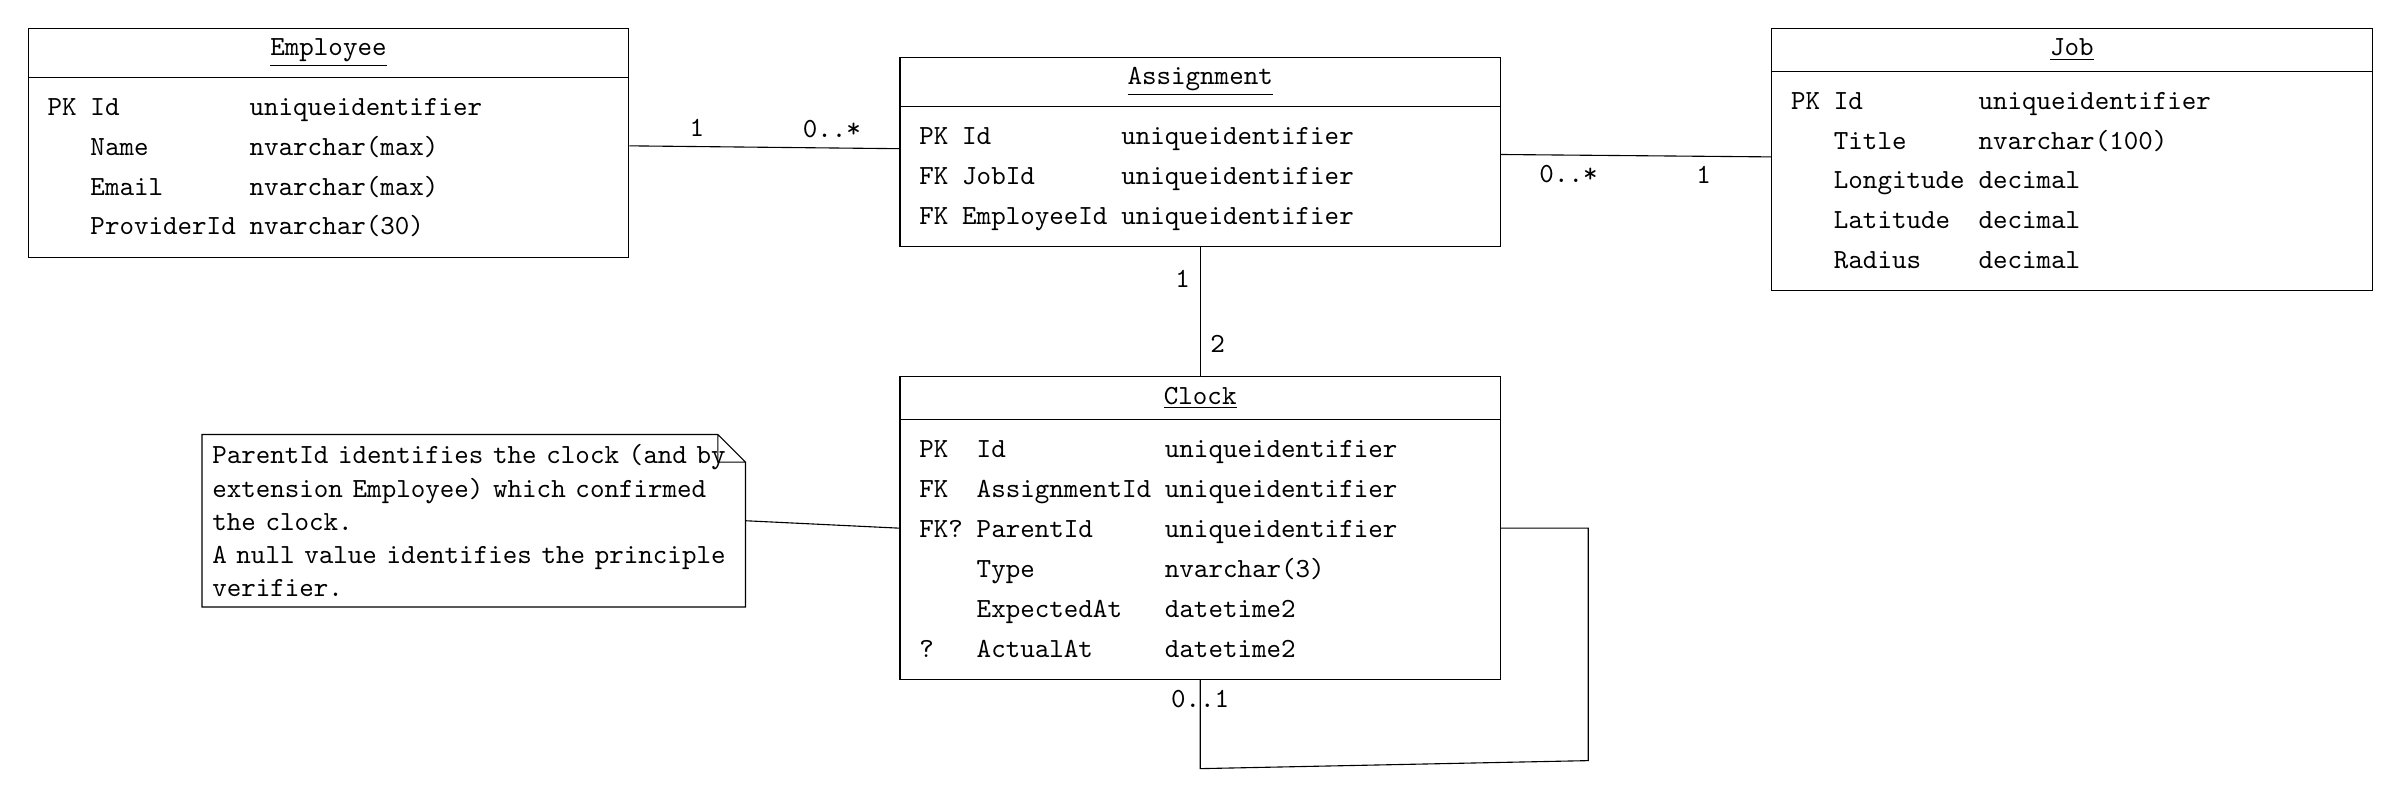
\begin{tikzpicture}
  \ttfamily

  \begin{object}[text width=20em]{Employee}{0,0}
    \attributes
    {
      PK & Id	         & uniqueidentifier \\
         & Name        & nvarchar(max) \\
         & Email       & nvarchar(max) \\
         & ProviderId  & nvarchar(30)
    }
  \end{object}


  \begin{object}[text width=20em]{Job}{60em,0}
    \attributes
    {
      PK  & Id	         & uniqueidentifier \\
          & Title        & nvarchar(100)    \\
          & Longitude    & decimal          \\
          & Latitude     & decimal          \\
          & Radius       & decimal
    }
  \end{object}

  \begin{object}[text width=20em]{Assignment}{30em,-1em}
    \attributes
    {
      PK & Id         & uniqueidentifier \\
      FK & JobId      & uniqueidentifier \\ 
      FK & EmployeeId & uniqueidentifier
    }
  \end{object}

  \begin{object}[text width=20em]{Clock}{30em,-12em}
    \attributes
    {
      PK  & Id           & uniqueidentifier \\
      FK  & AssignmentId & uniqueidentifier \\
      FK? & ParentId   & uniqueidentifier \\
          & Type       & nvarchar(3) \\
          & ExpectedAt & datetime2 \\
      ?   & ActualAt   & datetime2
    }
  \end{object}

  \association{Employee}{1}{}{Assignment}{0..*}{}
  \association{Job}{1}{}{Assignment}{0..*}{}
  \association{Clock}{}{2}{Assignment}{1}{}

  % clock self association
  \draw[-]
  (Clock.east) --
  ++(3em, 0) -- 
  ++(0, -8em) -- 
  (30em, -25.5em) -- % not janky at all
  (Clock.south);
  \node [below] at (Clock.south) {0..1};

  \umlnote [text width=18em] (note) at (5em,-14em) 
  {
    ParentId identifies the clock (and by extension
    Employee) which confirmed the clock.

    A null value identifies the principle verifier.
  };
  \draw[-] (note.east) -- (Clock.west);

\end{tikzpicture}
\end{document}
